% ================================================================= 11c
\section{Comparison with Zep}\label{sec:zep}

Graphiti's ingest makes several LLM calls per episode (about 6.9 million input tokens for one 115k-token history), so we
ran it on 10 LongMemEval questions, two per type, with every system ingesting on Haiku 5.5. The set was chosen around
questions \mx{} had missed in an earlier version, so it is not random and the differences are descriptive.

\begin{table}[!htb]
\centering\small
\setlength{\tabcolsep}{4pt}
\begin{tabular}{@{}l c r r r@{}}
\toprule
\thead{System} & \theadm{Correct\\/ 10} & \theadm{Memory\\tokens} & \theadm{Ingest\\\$ / question} & \theadm{LLM calls\\/ question}\\
\midrule
\mx{} ranked (4k) & \best{9} & \best{236} & 0.135 & 81 + 1,162 Jev\\ \rowrule
\mx{} full memory & \best{9} & 23,989 & 0.135 & 81 + 1,162 Jev\\ \rowrule
mem0 top-30 & 8 & 1,636 & \best{0.131} & 49\\ \rowrule
Zep + Jev & 6 & 2,369 & 0.60 & 153 + 381 Jev\\ \rowrule
Zep (LLM judge) & 5 & 2,311 & 0.71 & 452\\
\bottomrule
\end{tabular}
\caption{\textbf{10 LongMemEval questions, Haiku 5.5 extraction.} Ingest cost is metered per call. Jev requests cost
about \$0.00007 each.}
\label{tab:zep}
\end{table}

\begin{figure}[!htb]
\centering
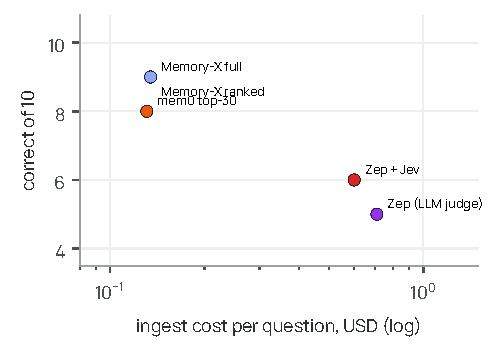
\includegraphics[width=0.55\linewidth]{figures/fig_zep.pdf}
\caption{\textbf{Correct answers against ingest cost} (log scale).}
\label{fig:zep}
\end{figure}

\mx{} answered 9 of 10 with ranked recall, against mem0's 8, with \textbf{6.9 times fewer memory tokens} and the same
ingest cost. Zep answered 5 with its LLM judge and 6 with Jev, at four to five times \mx{}'s ingest cost and with
blocks ten times larger. Routing Graphiti's judgement calls to Jev cut its cost by about a sixth. Graphiti asks two binary questions at
fixed thresholds and invalidates edges graph-wide; \mx{} asks a five-way question with per-outcome floors, guards and
scope-local corrections.
